\chapter{Design and Implementation}
% Justify design decisions, tools used, etc.
% NO CODE!!! (except for skeleton of algorithms maybe)

\section{Technologies used}

\subsection*{Haskell}
We have combined several technologies in order to create a nice workflow for our working environment. First of all, it is worth mentioning that we implemented the core algorithms for the neural network in Haskell. It is a very good candidate for solving mathematical problems, and has a strong type system that helped us detect bugs early on, at compile time, and made refactorings easy.

We also evaluated Python and Scala as our main implementation language for this project; Haskell was eventually chosen because of its strong, static type system (compared to Python), its easy integration with C (compared to Scala), and the personal learning interests of our team.

\subsection*{Image loading with C}
The functions responsible for image preprocessing (loading, rescaling, converting to gray-scale values, mapping pixels to binary patterns) were implemented in the \textbf{C} programming language, using the MagickWand ibrary which is part of ImageMagick. We used Haskell's \textit{Foreign Function Interface} for the communication between C and Haskell.

\subsection*{Git}
Since this was a group project in which all of us has to implement various parts of the system, we used Git as the version-control system that can keep track of our files, automatically merge source code and backup our data.

\subsection*{Test-driven development with QuickCheck}
Although Haskell as a programming language is already quite good at avoiding programming errors, it is not a theorem prover.
In our effort to keep our code correct and find errors early, we therefore maintained an extensive test suite structured with \textbf{Hspec}, where we performed both unit tests on lower level implementations and as well as behavioural tests testing the functionality of the full program.
We barely had to write tests in the example-driven style often found in imparative and dynamically typed languages, as we used \textbf{QuickCheck} to express the required functionality as lambda functions in first order logic. QuickCheck then generates thousands of tests cases automatically, based on the types our functions take as input, and also shrinks failing test cases to the smallest input that still fails. Using this technique, we found many failing edge cases in our initial implementation, and managed to keep the code size of our test suite small because most functions could be covered using only one or two first-order predicates.

%TODO. Talk about Jenkins , continuous integration, Review Board, ....
\subsection*{Code Reviews and Continuous Integration}
With the third year project being the largest group effort in our course, we tried to set ourselves new standards in using tools and techniques that help or benefit from the team. We set up an instance of the \textbf{ReviewBoard} web-based code review review system and enforced that all commits to our code base were reviewed by other team members before integration in the stable branch. We could avoid a lot of bugs with this and it also had the positive effect that the whole group agreed on the style and conceptual structure of the code.
We also set up our own \textbf{Jenkins} Continuous Integration server on a lab machine that pulled the code, built it and ran the test suite as soon as a change had been made; using this, we could get rapid feedback on new changes and whether they broke the build or introduced a correctness or performance regression. The code always being in a buildable state after every single commit also saved us from wasting time to manually find out afterwards what change broke it.



\section{Recognition System}

\begin{figure}[h]
  \centering
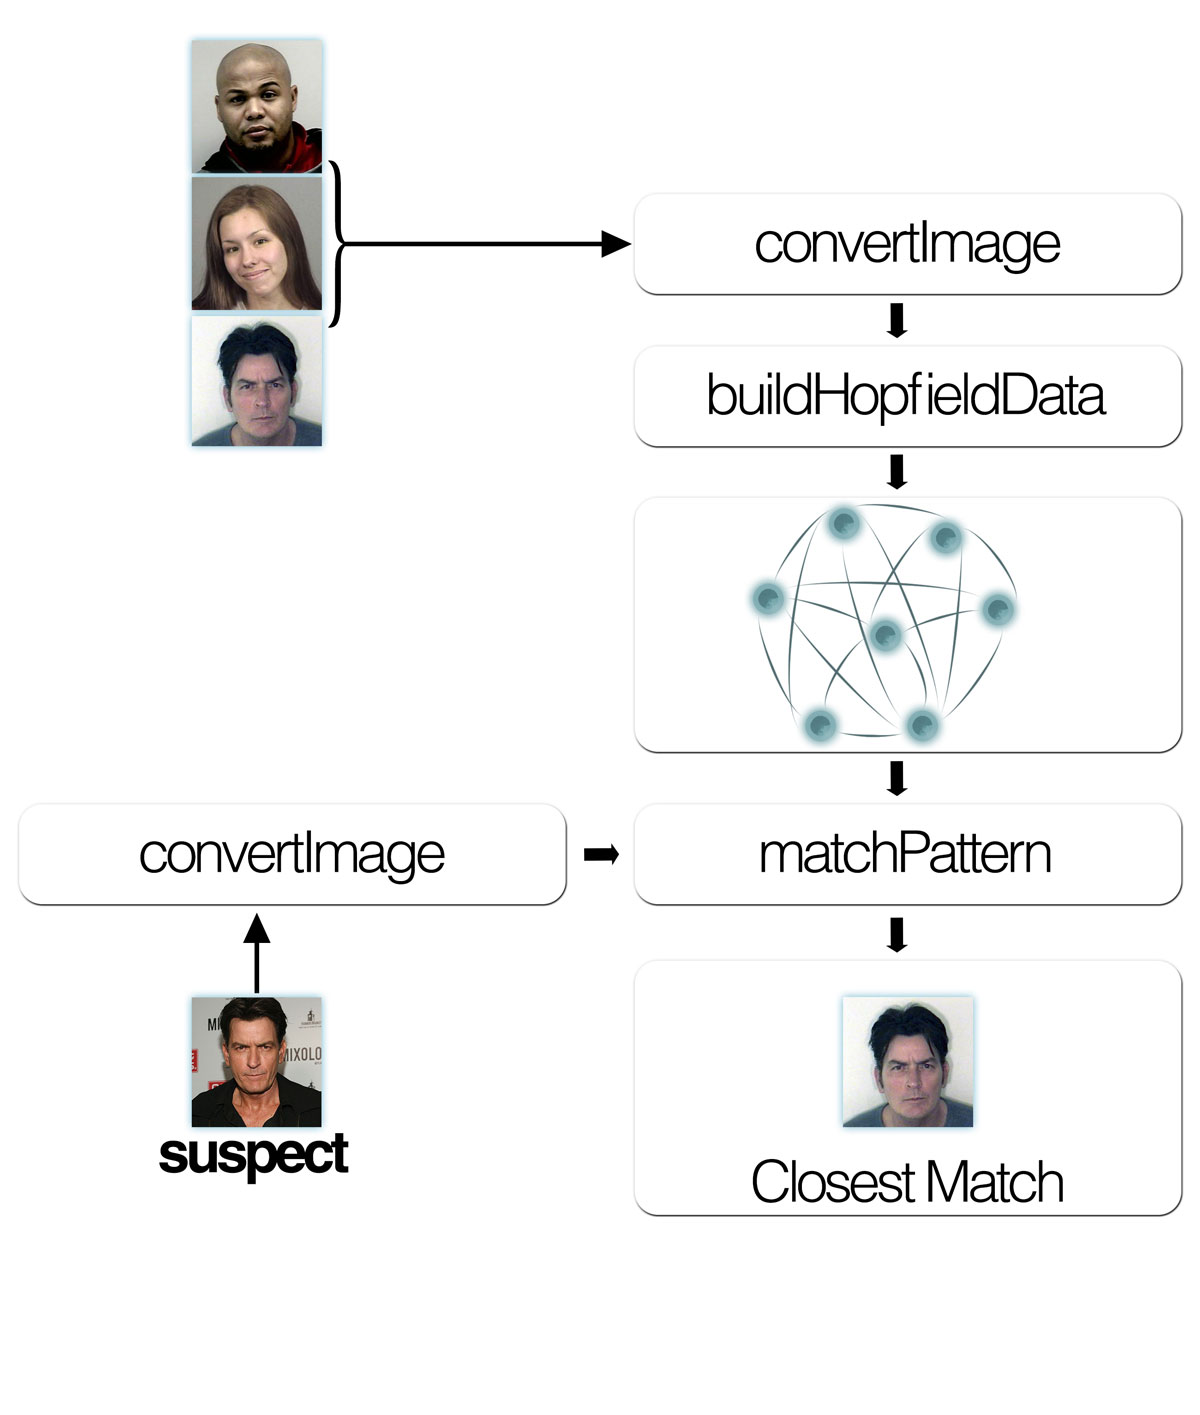
\includegraphics[scale=0.3]{recognition.jpg}
\caption{Outline of the Recognition System demonstrating how the various system components interact}
\label{fig:system}
\end{figure}




\section{Technical Challenges}

\subsection{Computation Time}


\hilight{maybe move detailed discussion to where the algorithm is actually described?}
The common theme of our experiments is measuring and comparing basins of attractions over a multitude of parameters, performed using the Storkey-Valabregue method (see \ref{storkey_basin_size}). As we know, this involves performing a very expensive computation: sampling 100 patterns for each Hamming radius, a maximum of N steps, and for each of those patterns iterative updates are run with the network until convergence is achieved. Though impossible due to properties of Hopfield networks, we can approximate the worst case complexity of the latter as requiring $2^N$ iterations until convergence, $2^N$ being the number of possible states. Thus we may cynically, for the sake of quantifying it, approximate the worst case complexity of the Storkey-Valabregue method to be $O(N2^N)$. While this is probably not an accurate representation of what occurs in practice, it serves to demonstrate the sheer amount of computation performed.

Naturally, this posed a significant computational challenge which we had to be overcome, as we typically obtain a large number of samples of basin measurements for our experiments, in the order of hundreds of samples for a given experiment. One way in which we overcome this limitation is by exploiting parallelism both at the process level (trivially achieved using \textbf{Haskell}!) and at the machine level, running multiple experiments on several lab machines. We also sought to improve the quality of our code itself, using profiling to identify hotspots. \hilight{next subsection on benchmarks}


\subsection{Big Data}

Another challenge which we have faced is dealing with the sheer amount of data generated by our experiments. The data typically needs to be collected, processed, and presented in a consistent manner. In order to address this issue, we attempted to automate such tasks. Automation is key, as it saves time, is not prone to (low level) human error, and generally scales well. Achieving this goal required the joint cooperation of three areas:

\begin{itemize}
\item Experiment executables should output data in a sensible and easy to parse format. Ideally, the output data should not be heavily processed so as to allow flexible use of it.

\item Writing scripts which format and aggregate data, typically calculating the mean value.

\item Presentation of data in the form of graphs of tables ought to be consistent. Ideally, the data should be kept separate from the format or design of its final presentation form. The \texttt{pgfplots} package for \LaTeX was very helpful for this.
\end{itemize}


\section{Anticipated Risks}

\subsection{Failure to match a pattern stored}
One of the risks associated with using the Hopfield model is that the converged pattern may not be one of the stored patterns, but rather a spurious pattern, as explained in section \ref{spurious_patterns}. This poses a problem for our recognition application, which needs to return as a result the closest matched stored pattern. Another issue with similar repercussions is that even after a large number of iterations are run, the pattern has not yet converged.
One solution to this \hilight{have we? also cross ref if applicable} is to simply output the closest stored pattern available. More precisely, the pattern that has the smallest Hamming distance between it and the current state of the system. This makes our image recognition robust to such unfortunate occurrences.


\subsection{A stored pattern not a fixed point}
It is possible that the given set of training patterns are such that some of the patterns simply cannot be ``stored'' in the network, i.e. it is not a fixed point of the network. The probability of this occurring increases as the relative number of training patterns with respect to the number of neurons increases \hilight{cross ref to capacity}.
The best way to deal with this problem is to perform a check (using \texttt{checkFixed}) \hilight{make sure we do that} and, if detected, report it  to the user and allow them to take action. The typical remedy for this would be to increase the number of neurons in the network, at the expense of increased resource usage in both space and time.


\subsection{Floating point calculation}
As we are dealing with extensive calculations of floating point value, we must be careful when dealing with such quantities. In particular, equality comparisons are likely to yield unexpected results. This has had an impact on some tests as well as functions such as \texttt{validWeights}. We have taken care of this problem by replacing equality comparisons and similar with fuzzy equality comparisons, with some accepted margin of error $\epsilon$.
